%%%%%%%%%%%%%%%%%%%%%%%%%%%%%%%%%%%%%%%
% Wenneker Resume/CV
% LaTeX Template
% Version 1.1 (19/6/2016)
%
% This template has been downloaded from:
% http://www.LaTeXTemplates.com
%
% Original author:
% Frits Wenneker (http://www.howtotex.com) with extensive modifications by
% Vel (vel@LaTeXTemplates.com) and Alexey Ermolenko (ermolenkoav@gmail.com)
%
% License:
% CC BY-NC-SA 3.0 (http://creativecommons.org/licenses/by-nc-sa/3.0/
%
%%%%%%%%%%%%%%%%%%%%%%%%%%%%%%%%%%%%%%

\documentclass[a4paper,12pt]{memoir} % Font and paper size
%%%%%%%%%%%%%%%%%%%%%%%%%%%%%%%%%%%%%%%%%
% Wenneker Resume/CV
% Structure Specification File
% Version 1.1 (19/6/2016)
%
% This file has been downloaded from:
% http://www.LaTeXTemplates.com
%
% Original author:
% Frits Wenneker (http://www.howtotex.com) with extensive modifications by 
% Vel (vel@latextemplates.com)
%
% License:
% CC BY-NC-SA 3.0 (http://creativecommons.org/licenses/by-nc-sa/3.0/)
%
%%%%%%%%%%%%%%%%%%%%%%%%%%%%%%%%%%%%%%%%%

%----------------------------------------------------------------------------------------
%	PACKAGES AND OTHER DOCUMENT CONFIGURATIONS
%----------------------------------------------------------------------------------------

\usepackage{XCharter} % Use the Bitstream Charter font
\usepackage[utf8]{inputenc} % Required for inputting international characters
\usepackage[T1]{fontenc} % Output font encoding for international characters

\usepackage[top=1cm,left=1cm,right=1cm,bottom=1cm]{geometry} % Modify margins

\usepackage{graphicx} % Required for figures

\usepackage{flowfram} % Required for the multi-column layout

\usepackage{hyperref} % URLs
\hypersetup{colorlinks=true,linkcolor=blue,urlcolor=blue}
\urlstyle{rm}

\usepackage[usenames,dvipsnames]{xcolor} % Required for custom colours

\usepackage{tikz} % Required for the horizontal rule

\usepackage{enumitem} % Required for modifying lists
\setlist{noitemsep,nolistsep} % Remove spacing within and around lists

\setlength{\columnsep}{\baselineskip} % Set the spacing between columns

% Define the left frame (sidebar)
\newflowframe{0.2\textwidth}{\textheight}{0pt}{0pt}[left]
\newlength{\LeftMainSep}
\setlength{\LeftMainSep}{0.2\textwidth}
\addtolength{\LeftMainSep}{1\columnsep}
 
% Small static frame for the vertical line
\newstaticframe{1.5pt}{\textheight}{\LeftMainSep}{0pt}
 
% Content of the static frame with the vertical line
\begin{staticcontents}{1}
\hfill
\tikz{\draw[loosely dotted,color=RoyalBlue,line width=1.5pt,yshift=0](0,0) -- (0,\textheight);}
\hfill\mbox{}
\end{staticcontents}
 
% Define the right frame (main body)
\addtolength{\LeftMainSep}{1.5pt}
\addtolength{\LeftMainSep}{1\columnsep}
\newflowframe{0.7\textwidth}{\textheight}{\LeftMainSep}{0pt}[main01]

\pagestyle{empty} % Disable all page numbering

\setlength{\parindent}{0pt} % Stop paragraph indentation

%----------------------------------------------------------------------------------------
%	NEW COMMANDS
%----------------------------------------------------------------------------------------

\newcommand{\userinformation}[1]{\renewcommand{\userinformation}{#1}} % Define a new command for the CV user's information that goes into the left column

\newcommand{\cvheading}[1]{{\Huge\bfseries\color{RoyalBlue} #1} \par\vspace{.6\baselineskip}} % New command for the CV heading
\newcommand{\cvsubheading}[1]{{\Large\bfseries #1} \bigbreak} % New command for the CV subheading

\newcommand{\Sep}{\vspace{1em}} % New command for the spacing between headings
\newcommand{\SmallSep}{\vspace{0.5em}} % New command for the spacing within headings

\newcommand{\aboutme}[2]{ % New command for the about me section
\textbf{\color{RoyalBlue} #1}~~#2\par\Sep
}
	
\newcommand{\CVSection}[1]{ % New command for the headings within sections
{\Large\textbf{#1}}\par
\SmallSep % Used for spacing
}

\newcommand{\CVItem}[2]{ % New command for the item descriptions
\textbf{\color{RoyalBlue} #1}\par
#2
\SmallSep % Used for spacing
}

\newcommand{\bluebullet}{\textcolor{RoyalBlue}{$\circ$}~~} % New command for the blue bullets
 % Include the file specifying document layout and packages

\userinformation{ % Set the content that goes into the sidebar of each page
    \begin{flushright}
% Comment out this figure block if you don't want a photo
        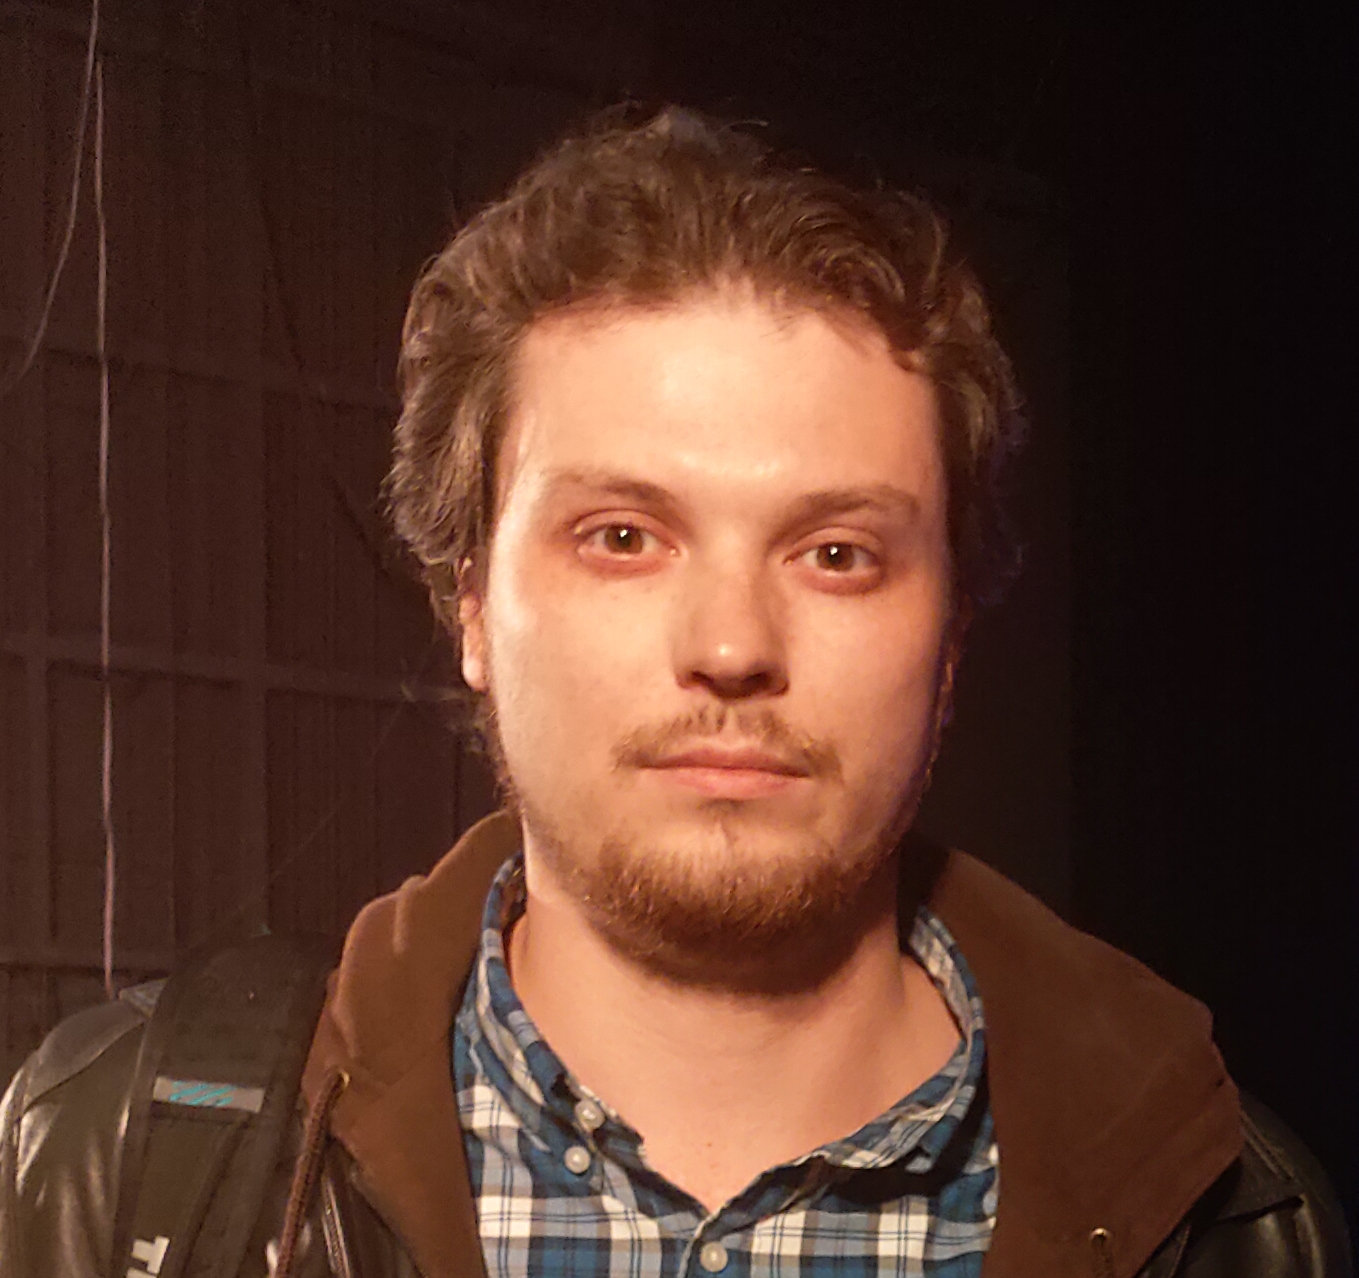
\includegraphics[width=1\columnwidth]{photo}\\[\baselineskip] % Your photo
        \small % Smaller font size
        \textbf{Контакты} \\ % Name
        \href{https://github.com/ermolenkoav}{GitHub} \\
        \href{https://ermolenkoav.t.me/}{Telegram} \\ % Email
        \href{https://www.linkedin.com/in/ermolenkoav/}{LinkedIn} \\ % Your URL
        \href{mailto:ermolenkoav@gmail.com}{Email} \\ % Email
        +7 (918) 565--36--01 \\ % Your phone number
        \Sep % Some whitespace
        \textbf{Адрес} \\
        Ростов-на-Дону, Россия \\
        \vfill % Whitespace under this block to push it up under the photo
    \end{flushright}
}

%----------------------------------------------------------------------------------------
\begin{document}
    \userinformation % Print your information in the left column
    \framebreak % End of the first column

%----------------------------------------------------------------------------------------
%	HEADING
%----------------------------------------------------------------------------------------

    \cvheading{Алексей Ермоленко}
    \cvsubheading{Инженер программист}

%----------------------------------------------------------------------------------------
%	ABOUT ME
%----------------------------------------------------------------------------------------

    \aboutme{Обо мне}{Активно участвовал во всех этапах жизненного цикла разработки программного и аппаратного обеспечения
    для сбора и обработки больших данных. В том числе: разработка высоконагруженных back-end микросервисов, проектирование SQL и NoSQL баз данных
    проектирование структур, клиент-серверного и встраиваемого ПО по заказу клиента, эффективное использование ограниченных вычислительных ресурсов,
    поддержка и рефакторинг больших кодовых баз, внедрение новых технологий и подходов. Написание проектной и сопроводительной документации по разработке.
    Участвовал в презентационных мероприятиях: \href{https://youtu.be/1QDFi3-sKCY}{Living Sensors}}

%----------------------------------------------------------------------------------------
%	SKILLS
%----------------------------------------------------------------------------------------

    \CVSection{Навыки}

    \CVItem{Разработка}
    {\begin{tabular}{ l l l l l }
         \bluebullet Golang & \bluebullet SQL & \bluebullet C/C++ & \bluebullet Python & \bluebullet Java \\
    \end{tabular}}

    \CVItem{Администрирование}
    {\begin{tabular}{ l l l }
         \bluebullet Docker & \bluebullet Docker Compose & \bluebullet K8s \\
    \end{tabular}}

%----------------------------------------------------------------------------------------
%	EXPERIENCE
%----------------------------------------------------------------------------------------

    \CVSection{Опыт работы}

    \CVItem{Октябрь 2022 - По текущий момент, \textit{Разработчик}, WB Tech ООО.}{
        \begin{itemize}
            \item Разработал на основе кластера ClichHouse NoSQL базу данных для хранения и анализа финансовых данных.
            \item Заменил кластер NATS на кластер Kafka в высоконагруженном проекте.
            \item Участвовал в запуске нового отдела компании.
            \begin{itemize}
                \item Golang - fasthttp,pgx,clickhouse-go e.t.c
            \end{itemize}
            \item Разработал дизайн баз данных аналитической финансовой системы.
            \begin{itemize}
                \item ClickHouse NoSQL
            \end{itemize}
        \end{itemize}
    }

    \CVItem{Октябрь 2021 - Июнь 2022, \textit{Ведущий инженер}, DDoS-Guard ltd.}{
        \begin{itemize}
            \item Занимался поддержкой и внедрением нового функционала в высоконагруженный реверспрокси.
            \begin{itemize}
                \item C++ - STL, Boost, GoogleTest
            \end{itemize}
            \item Участвовал в старте разработки первоначального функционала l4 балансировщика нагрузки.
            \begin{itemize}
                \item Linux/eBPF, Golang/\href{https://github.com/cilium/ebpf}{Cilium eBPF}
            \end{itemize}
            \item Участвовал в написании технической документации.
            \begin{itemize}
                \item \href{Diagrams.net}{Draw.io}, \LaTeX{},
            \end{itemize}
        \end{itemize}
    }

    \CVItem{Февраль 2020 - Октябрь 2021, \textit{Инженер программист}, ООО Ростпэй}{
        \begin{itemize}
            \item Занимался разработкой клиент-серверных приложений.
            \begin{itemize}
                \item C++, STL, \href{https://github.com/pocoproject/poco}{POCO Libraries}, wxWidgets, GoogleTest, Win32, Design patterns
            \end{itemize}
            \item Костомизация браузера Chromium.
            \begin{itemize}
                \item C++ - STL, Chromium, Работа с большой кодовой базой.
            \end{itemize}
            \item Участвовал в написании технической документации проекта.
            \begin{itemize}
                \item \href{Diagrams.net}{Draw.io}
            \end{itemize}
        \end{itemize}
    }

%----------------------------------------------------------------------------------------
%	NEW PAGE DELIMITER
%	Place this block wherever you would like the content of your CV to go onto the next page
%----------------------------------------------------------------------------------------

    \clearpage % Start a new page
    \userinformation % Print your information in the left column
    \framebreak % End of the first column

%----------------------------------------------------------------------------------------

    \CVItem{Ноябрь 2017 - Январь 2020, \textit{Младший научный сотрудник}, НИТЦ нейротехнологий, Южный Федеральный Университет.}{
        \begin{itemize}
            \item Занимался разработкой програмного обеспечения для управления экспериментами
            \begin{itemize}
                \item C/C++ - STL, Qt Widgets, Boost, GoogleTest, Win32
            \end{itemize}
            \item Разрабатывал электронные устройства электромиостимуляции и миостимуляции.
            \begin{itemize}
                \item Texas Instruments CC2541,CC2540, Altium Designer, Atmel AVR
            \end{itemize}
            \item Участвовал в написании технической документации проекта
        \end{itemize}
    }

    \CVItem{Февраль 2015 - Октябрь 2017, \textit{Инженер программист}, ООО Дон-страйк}{
        \begin{itemize}
            \item Разрабатывал электронные устройства и программное обеспечение управления экспериментом.
            \begin{itemize}
                \item C/C++ - STL, Qt
                \item Texas Instruments CC2541,CC2540, Altium Designer, Atmel AVR
            \end{itemize}
            \item Участвовал в написании технической документации проекта.
            \begin{itemize}
                \item \LaTeX{}
            \end{itemize}
        \end{itemize}
    }

    \CVItem{Сентябрь 2013 - Февраль 2015, \textit{Инженер программисть}, ФГАНУ НИИ Спецвузавтоматика}{
        \begin{itemize}
            \item Участвовал в разработке электронных устройств и программного обеспечения.
            \begin{itemize}
                \item C/C++
                \item Atmel AVR, Atmel Designer
            \end{itemize}
            \item Участвовал в написании технической документации проекта.
        \end{itemize}
    }

    \tiny

%----------------------------------------------------------------------------------------
%	EDUCATION
%----------------------------------------------------------------------------------------
    \CVSection{Образование}
    \CVItem{2011 - 2014, Южный Федеральный Университет}{Факультет физики, Аспирантура}

    \CVItem{2006 - 2011, Южный Федеральный Университет}{Факультет физики, Медицинская физика, Специалитет}
    \Sep % Extra whitespace after the end of a section

%----------------------------------------------------------------------------------------
%	LANGUAGE SKILLS
%----------------------------------------------------------------------------------------
    \CVSection{Языки}
    \CVItem{English}{B1 Strong Pre-Intermediate}
    \Sep % Extra whitespace after the end of a section

%----------------------------------------------------------------------------------------
%	NEW PAGE DELIMITER
%	Place this block wherever you would like the content of your CV to go onto the next page
%----------------------------------------------------------------------------------------
%\clearpage % Start a new page
%\userinformation % Print your information in the left column
%\framebreak % End of the first column

%----------------------------------------------------------------------------------------
%	AWARDS
%----------------------------------------------------------------------------------------
    \CVSection{Награды}
    \CVItem{2022, ООО DDoS-Guard}{За креативность и нестандартность мышления в решении поставленных задач}

    \CVItem{2010, \textit{Факультет Физики}, Южный Федеральный Университет}{Лауреат 62й Студенческой Научной Конференции ЮФУ}
    \Sep % Extra whitespace after the end of a section

%----------------------------------------------------------------------------------------
%	ADVANCED TRAINING, COURSES
%----------------------------------------------------------------------------------------
    \CVSection{Курсы}
    \CVItem{2018, Otus}{Разработчик C++}

%\CVItem{2020, Otus}{Spring Framework Developer}
%\Sep % Extra whitespace after the end of a section

%----------------------------------------------------------------------------------------
%	INTERESTS
%----------------------------------------------------------------------------------------
    \CVSection{Интересы}
    \CVItem{Профессиональные}{Разработка программного обеспечения, разработка электронных устройств}

    \CVItem{Личные}{Пешие прогулки по горам}
    \Sep % Extra whitespace after the end of a section

%---------------------------------------------------------------------------------------
\end{document}